% Soubory musí být v kódování, které je nastaveno v příkazu \usepackage[...]{inputenc}

\documentclass[%        Základní nastavení
  %draft,    				  % Testovací překlad
  12pt,       				% Velikost základního písma je 12 bodů
	t,                  % obsah slajdů bude vždy začínat od shora (nebude vertikálně centrovaný)
	aspectratio=1610,   % poměr stran bude 16:10 (všechny projektory v učebnách na Technické 12 Brno),
	                    % další volby jsou 43, 149, 169, 54, 32.
	unicode,						% Záložky a informace budou v kódování unicode
]{beamer}				    	% Dokument třídy 'zpráva', vhodná pro sazbu závěrečných prací s kapitolami
%\usepackage{etex}

\usepackage[utf8]		  % Kódování zdrojových souborů je v UTF-8
	{inputenc}					% Balíček pro nastavení kódování zdrojových souborů
	
\usepackage{graphicx} % Balíček 'graphicx' pro vkládání obrázků
											% Nutné pro vložení logotypů školy a fakulty

\usepackage[          % Balíček 'acronym' pro sazby zkratek a symbolů
	nohyperlinks				% Nebudou tvořeny hypertextové odkazy do seznamu zkratek
]{acronym}						
											% Nutné pro použití prostředí 'acronym' balíčku 'thesis'

%% Balíček hyperref je volán třídou beamer automaticky, proto není třeba následujícího kódu:
%\usepackage[
%	breaklinks=true,		% Hypertextové odkazy mohou obsahovat zalomení řádku
%	hypertexnames=false % Názvy hypertextových odkazů budou tvořeny
%											% nezávisle na názvech TeXu
%]{hyperref}						% Balíček 'hyperref' pro sazbu hypertextových odkazů
%											% Nutné pro použití příkazu 'nastavenipdf' balíčku 'thesis'

\usepackage{cmap} 		% Balíček cmap zajišťuje, že PDF vytvořené `pdflatexem' je
											% plně "prohledávatelné" a "kopírovatelné"

%\usepackage{upgreek}	% Balíček pro sazbu stojatých řeckých písmem
											%% např. stojaté pí: \uppi
											%% např. stojaté mí: \upmu (použitelné třeba v mikrometrech)
											%% pozor, grafická nekompatibilita s fonty typu Computer Modern!

%\usepackage{amsmath} %balíček pro sabu náročnější matematiky

\usepackage{booktabs} % Balíček, který umožňuje v tabulce používat
                      % příkazy \toprule, \midrule, \bottomrule


%%%%%%%%%%%%%%%%%%%%%%%%%%%%%%%%%%%%%%%%%%%%%%%%%%%%%%%%%%%%%%%%%
%%%%%%      Definice informací o dokumentu             %%%%%%%%%%
%%%%%%%%%%%%%%%%%%%%%%%%%%%%%%%%%%%%%%%%%%%%%%%%%%%%%%%%%%%%%%%%%

\input{nastaveni}      % v tomto souboru doplňte údaje o sobě, o názvu práce...
                       % (tento soubor je sdílený s textem práce)

%%%%%%%%%%%%%%%%%%%%%%%%%%%%%%%%%%%%%%%%%%%%%%%%%%%%%%%%%%%%%%%%%%%%%%%%

%%%%%%%%%%%%%%%%%%%%%%%%%%%%%%%%%%%%%%%%%%%%%%%%%%%%%%%%%%%%%%%%%%%%%%%%
%%%%%%     Nastavení polí ve Vlastnostech dokumentu PDF      %%%%%%%%%%%
%%%%%%%%%%%%%%%%%%%%%%%%%%%%%%%%%%%%%%%%%%%%%%%%%%%%%%%%%%%%%%%%%%%%%%%%
%% Při vloženém balíčku 'hyperref' lze použít příkaz '\pdfsettings'
\pdfsettings
%  Nastavení polí je možné provést také ručně příkazem:
%\hypersetup{
%  pdftitle={Název studentské práce},    	% Pole 'Document Title'
%  pdfauthor={Autor studenstké práce},   	% Pole 'Author'
%  pdfsubject={Typ práce}, 						  	% Pole 'Subject'
%  pdfkeywords={Klíčová slova}           	% Pole 'Keywords'
%}
\hypersetup{pdfpagemode=FullScreen}       % otevření rovnou v režimu celé obrazovky
%%%%%%%%%%%%%%%%%%%%%%%%%%%%%%%%%%%%%%%%%%%%%%%%%%%%%%%%%%%%%%%%%%%%%%%

\usetheme{VUT} 				% barvy a rozložení prezentace odpovídající VUT FEKT
% alternativně lze použít jiná berevná témata, ale bez záruky. Například: 
%\usetheme{Darmstadt} \usecolortheme{default2}
\logoheader					% vytvoření zkráceného loga VUT FEKT v hlavičce slajdu, nechte odkomentované



\begin{document}

% v případě zakomentování následujícího se zobrazí v pravém dolním rohu slajdů klikatelné navigační symboly 
\disablenavigationsymbols

% titulní snímek, vysazen bez horních, dolních a postranních lišt (volba plain),
% není tak vysazen ani nadpis snímku
\maketitle

%%%%%%%%%%%%%%%%%%%%%%%%%%%%%%%%%%%%%%%%%%%%%%%%%%%%%%%%%%%%%%%%%%%%%%%

\begin{frame} 
	% nadpis snímku
	\frametitle{Cíle práce}
	\begin{figure}[ht!]
		\centering
		\begin{minipage}{0.3\textwidth}
			\vspace*{-3cm}
			\begin{itemize}
				\item ICT tester
				\item Fixture
				\item Měření odporu
				\item Testovací jehly
				\item Probes
				\item bRC
			\end{itemize}
		\end{minipage}
		\begin{minipage}{0.65\textwidth}
		\includegraphics[height = 0.8\textheight]{obrazky/ICT_tester.png}
		\end{minipage}
	\end{figure}
\end{frame}

\begin{frame} 
	% nadpis snímku
	\frametitle{Koncepce testeru 1/2}
	\vspace*{0.5cm}
	\begin{figure}[ht!]
		\centering
		%\includegraphics[width = \textwidth]{obrazky/system_connection.png}
		\includegraphics[width = \textwidth]{obrazky/system_connection_and_fixture.png}
	\end{figure}
\end{frame}

\begin{frame} 
	% nadpis snímku
	\frametitle{Koncepce testeru 2/2}
	\vspace*{0.5cm}
	\begin{figure}[ht!]
		\centering
		%\includegraphics[width = \textwidth]{obrazky/system_connection.png}
		\includegraphics[width = \textwidth]{obrazky/telnet_http_pc.png}
	\end{figure}
\end{frame}


\begin{frame} 
	% nadpis snímku
	\frametitle{Měřící karta 1/4}
	\vspace*{0.7cm}
	\begin{figure}[ht!]
		\centering
		%\includegraphics[width = \textwidth]{obrazky/system_connection.png}
		\includegraphics[width = \textwidth]{obrazky/karta_3D_NP.png}
	\end{figure}
\end{frame}

\begin{frame} 
	% nadpis snímku
	\frametitle{Měřící karta  2/4}
	\vspace*{0.5cm}
	\begin{figure}[ht!]
		\centering
		%\includegraphics[width = \textwidth]{obrazky/system_connection.png}
		\includegraphics[width = \textwidth]{obrazky/karta_system_diagram.png}
	\end{figure}
\end{frame}


\begin{frame} 
	% nadpis snímku
	\frametitle{Měřící karta 3/4}
	\vspace*{0.5cm}
	\begin{figure}[ht!]
		\centering
		%\includegraphics[width = \textwidth]{obrazky/system_connection.png}
		\includegraphics[width = \textwidth]{obrazky/2_and_4_pins_connection.png}
	\end{figure}
\end{frame}

\begin{frame} 
	% nadpis snímku
	\frametitle{Měřící karta 4/4}
	\vspace*{0.5cm}
	\begin{figure}[ht!]
		\centering
		%\includegraphics[width = \textwidth]{obrazky/system_connection.png}
		\includegraphics[width = \textwidth]{obrazky/final_connection.png}
	\end{figure}
\end{frame}

\begin{frame} 
	% nadpis snímku
	\frametitle{Volba Rx}
	\begin{figure}[ht!]

$\frac{V_{ref}}{2^{12}} + \frac{V_{in} \cdot R^P_{DSon}}{R_{out}/N_{pins} + R^P_{DSon}} < \left| \frac{\partial V_{out} }{\partial R_{path}}\cdot \Delta R_{path} \right|$
		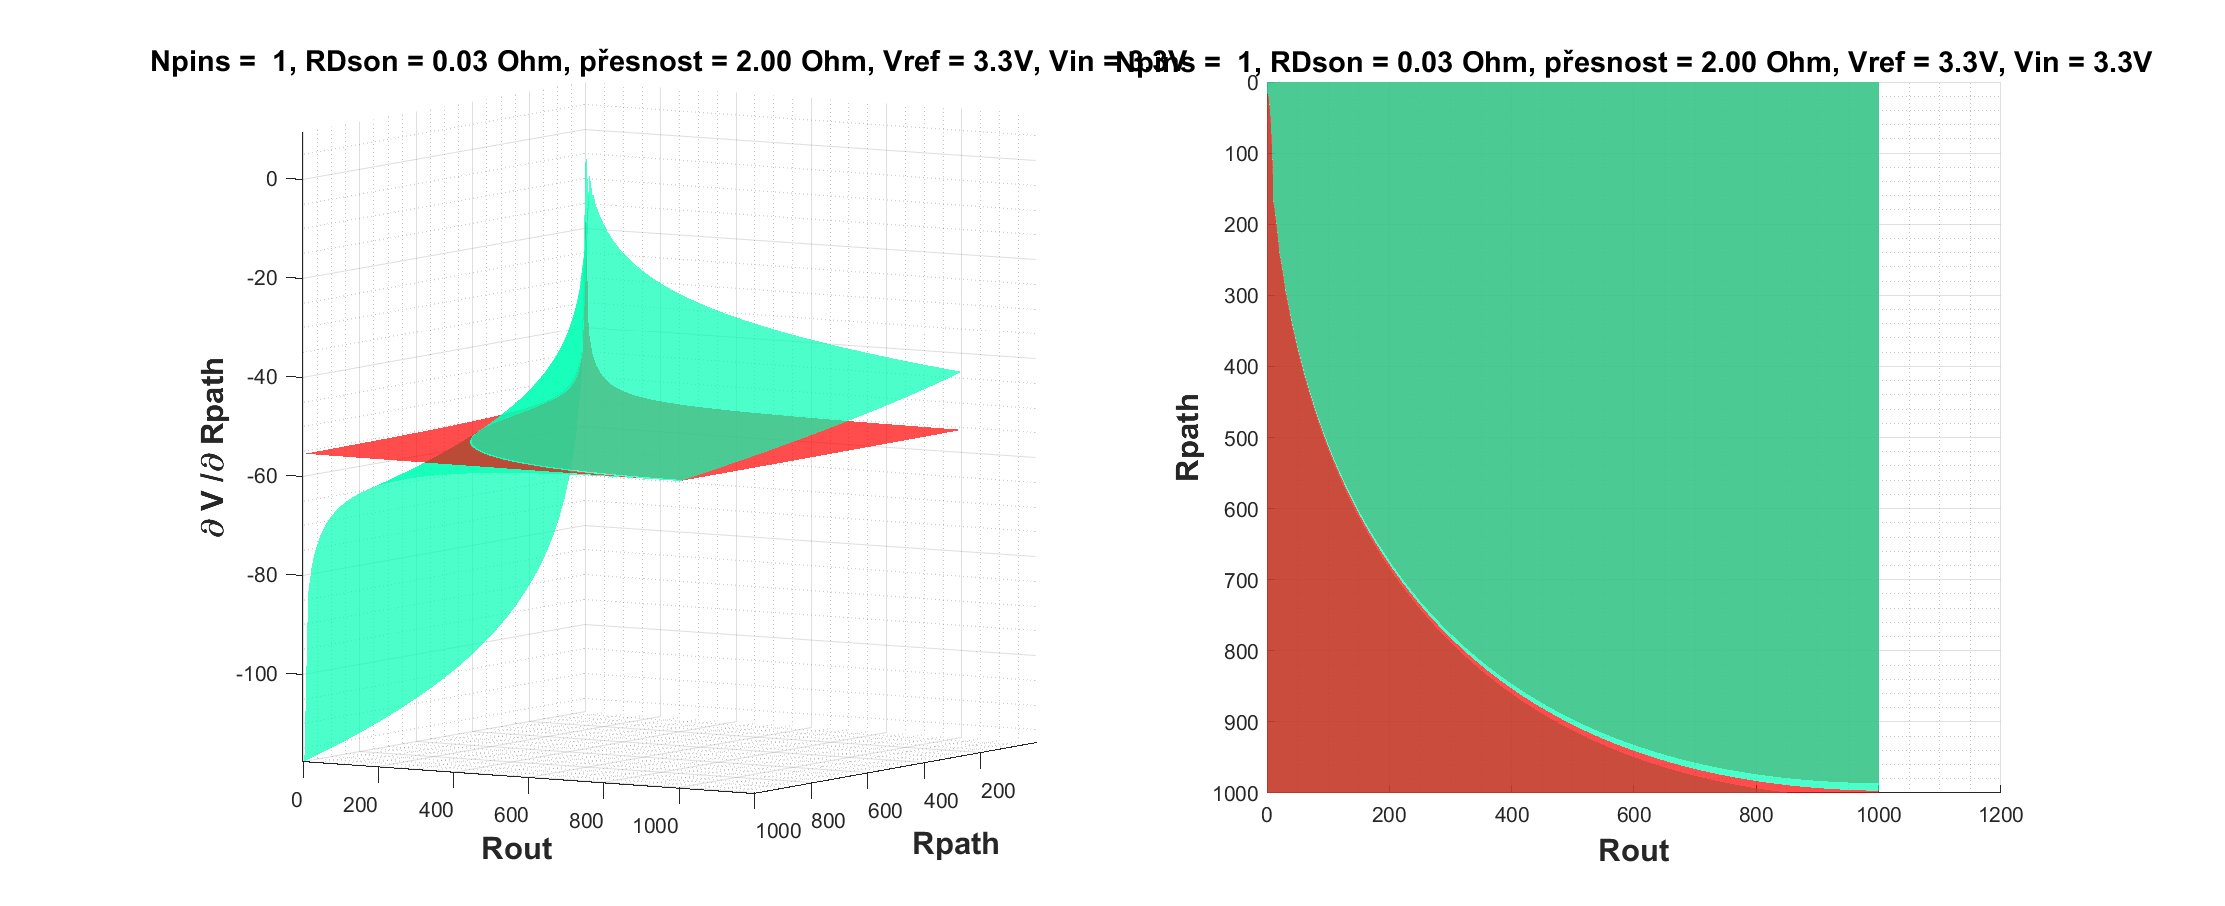
\includegraphics[height = 0.6\textheight]{obrazky/general_dVF.eps}
	\end{figure}
\end{frame}

\begin{frame} 
	% nadpis snímku
	\frametitle{Volba Rx: vliv paralelních cest}
	\begin{figure}[ht!]
		\centering
		\begin{minipage}{0.3\textwidth}
			\begin{itemize}
				\item 1 až 80 pinů
				\item přesnost 2\,$\Omega$
			\end{itemize}
		\end{minipage}
		\begin{minipage}{0.65\textwidth}
		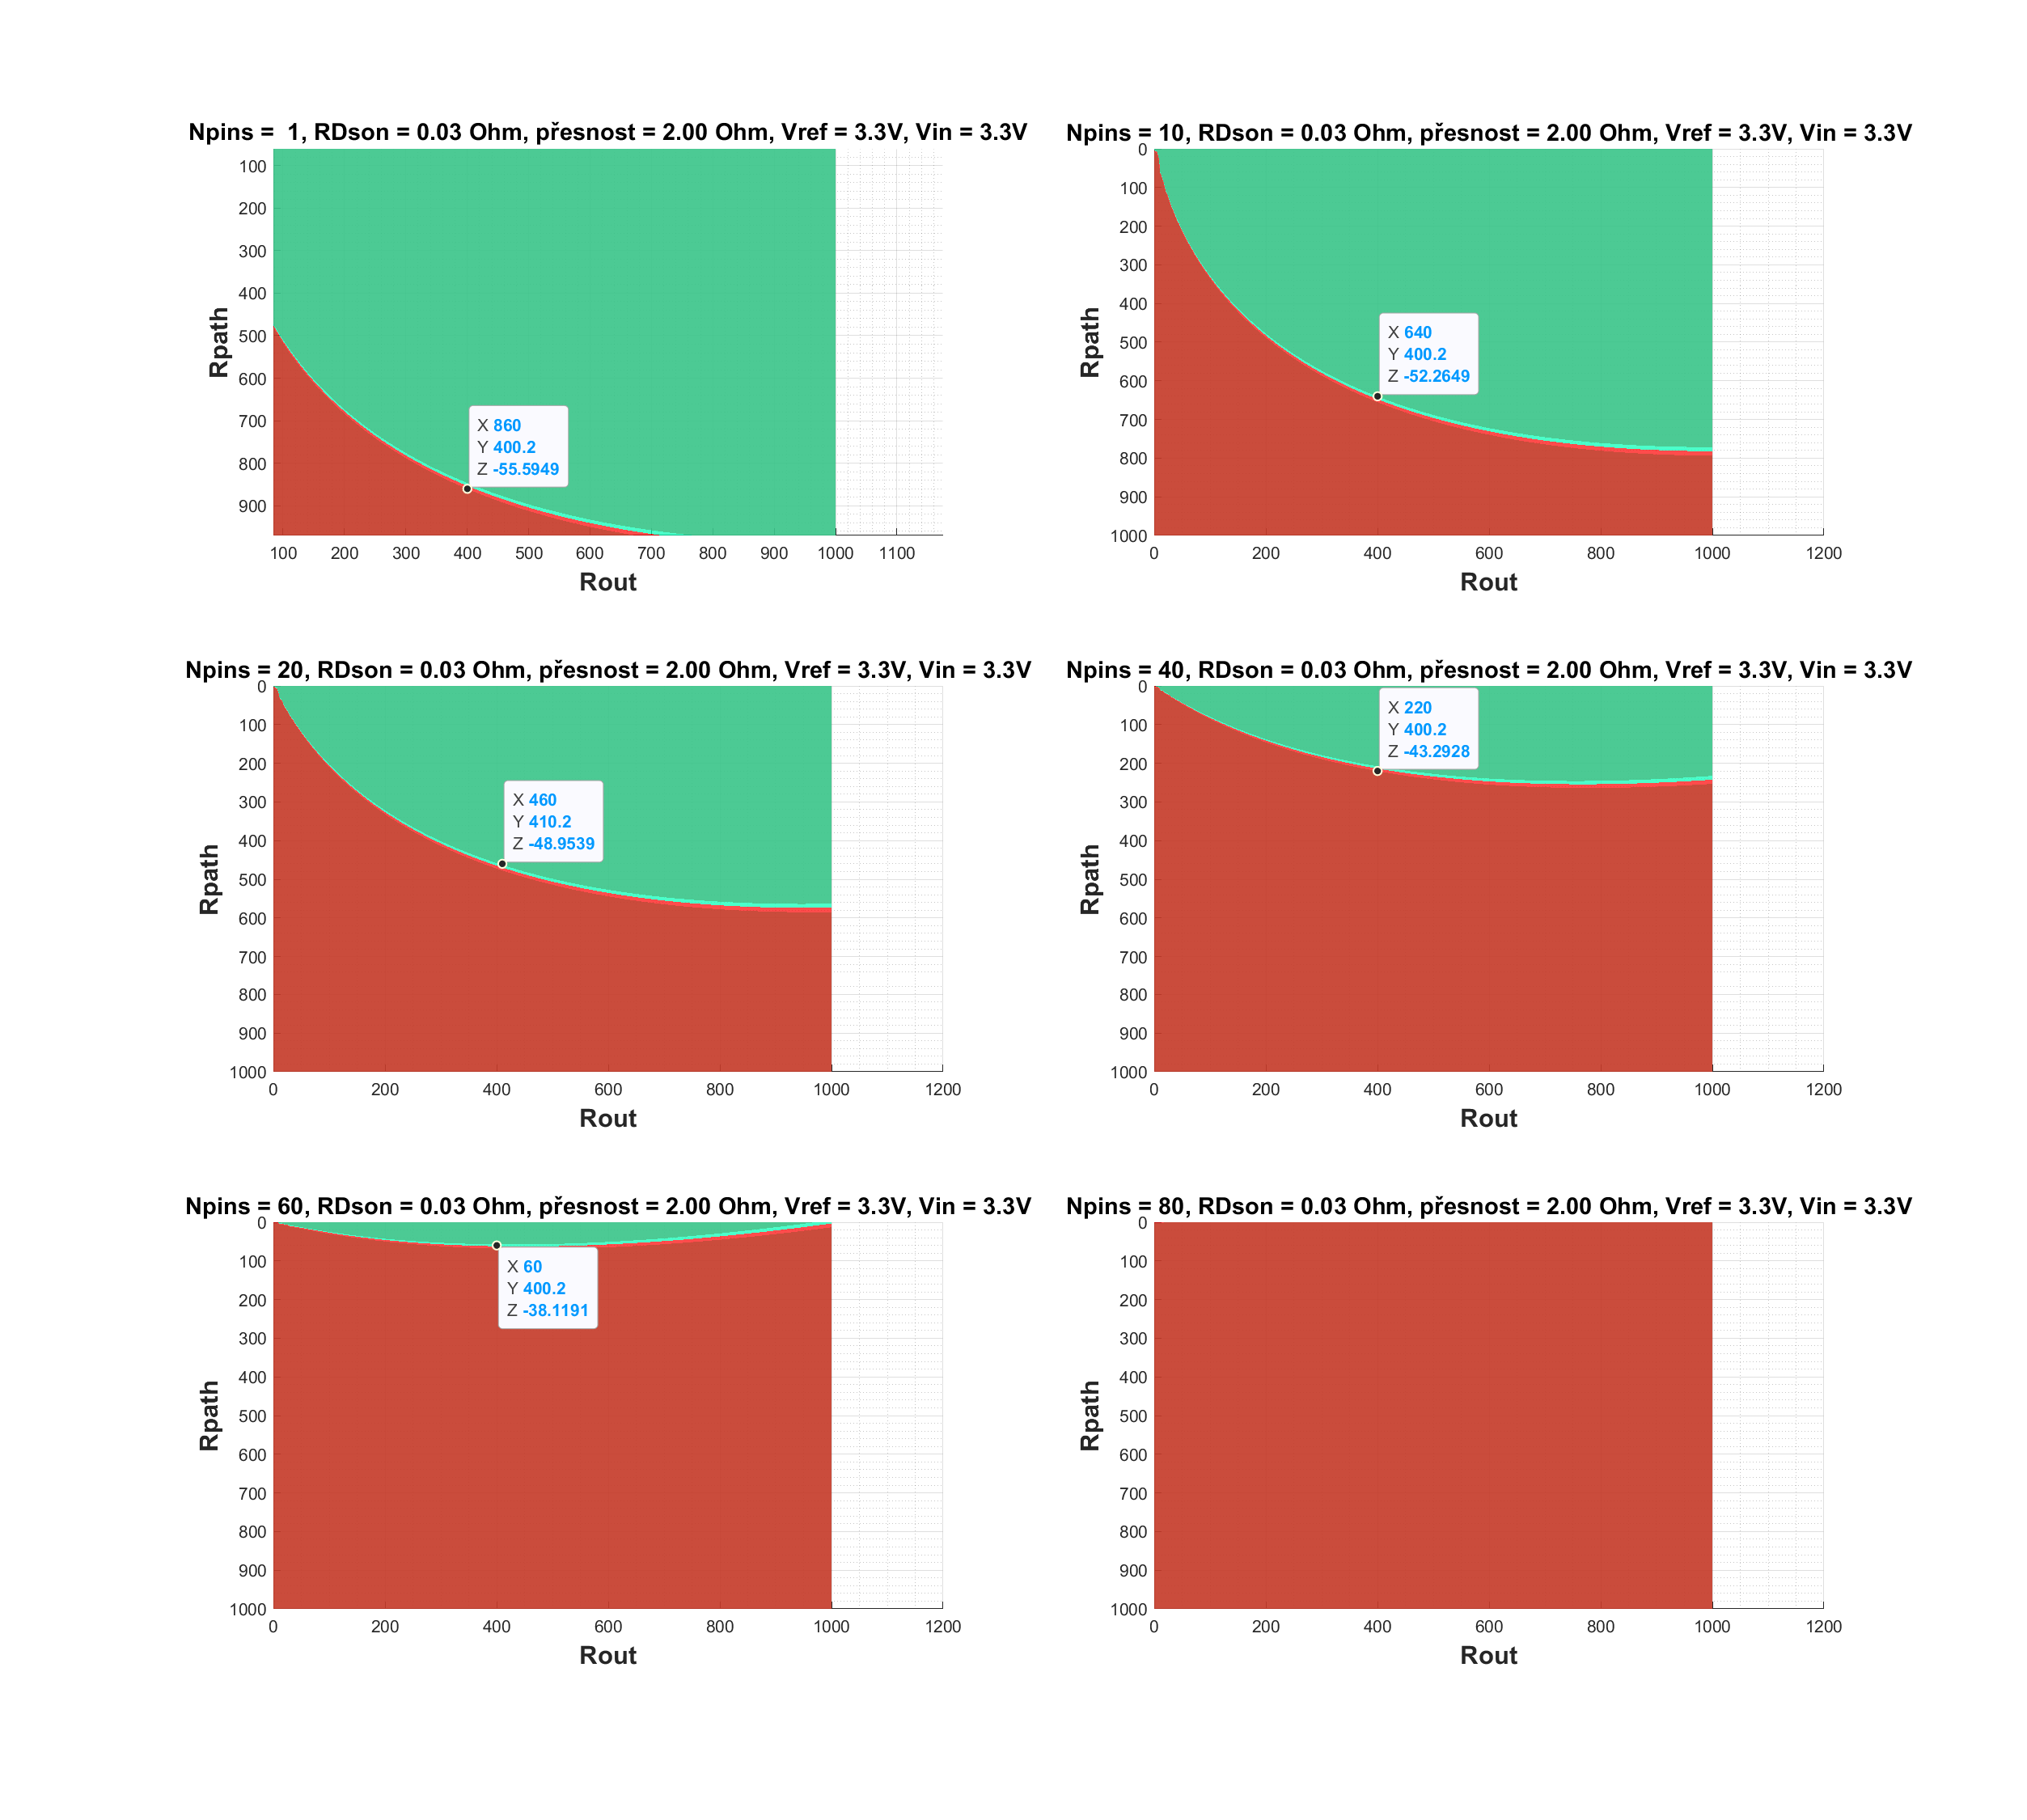
\includegraphics[height = 0.8\textheight]{obrazky/PASS_FAIL_MERENI.eps}
		\end{minipage}
	\end{figure}
\end{frame}


\begin{frame} 
	% nadpis snímku
	\frametitle{Volba Rx: Maximální přesnost}
	\begin{figure}[ht!]
		\centering
		\begin{minipage}{0.3\textwidth}
			\begin{itemize}
				\item pouze 1 pin
				\item přesnost 0.03 - 1\,$\Omega$
			\end{itemize}
		\end{minipage}
		\begin{minipage}{0.65\textwidth}
		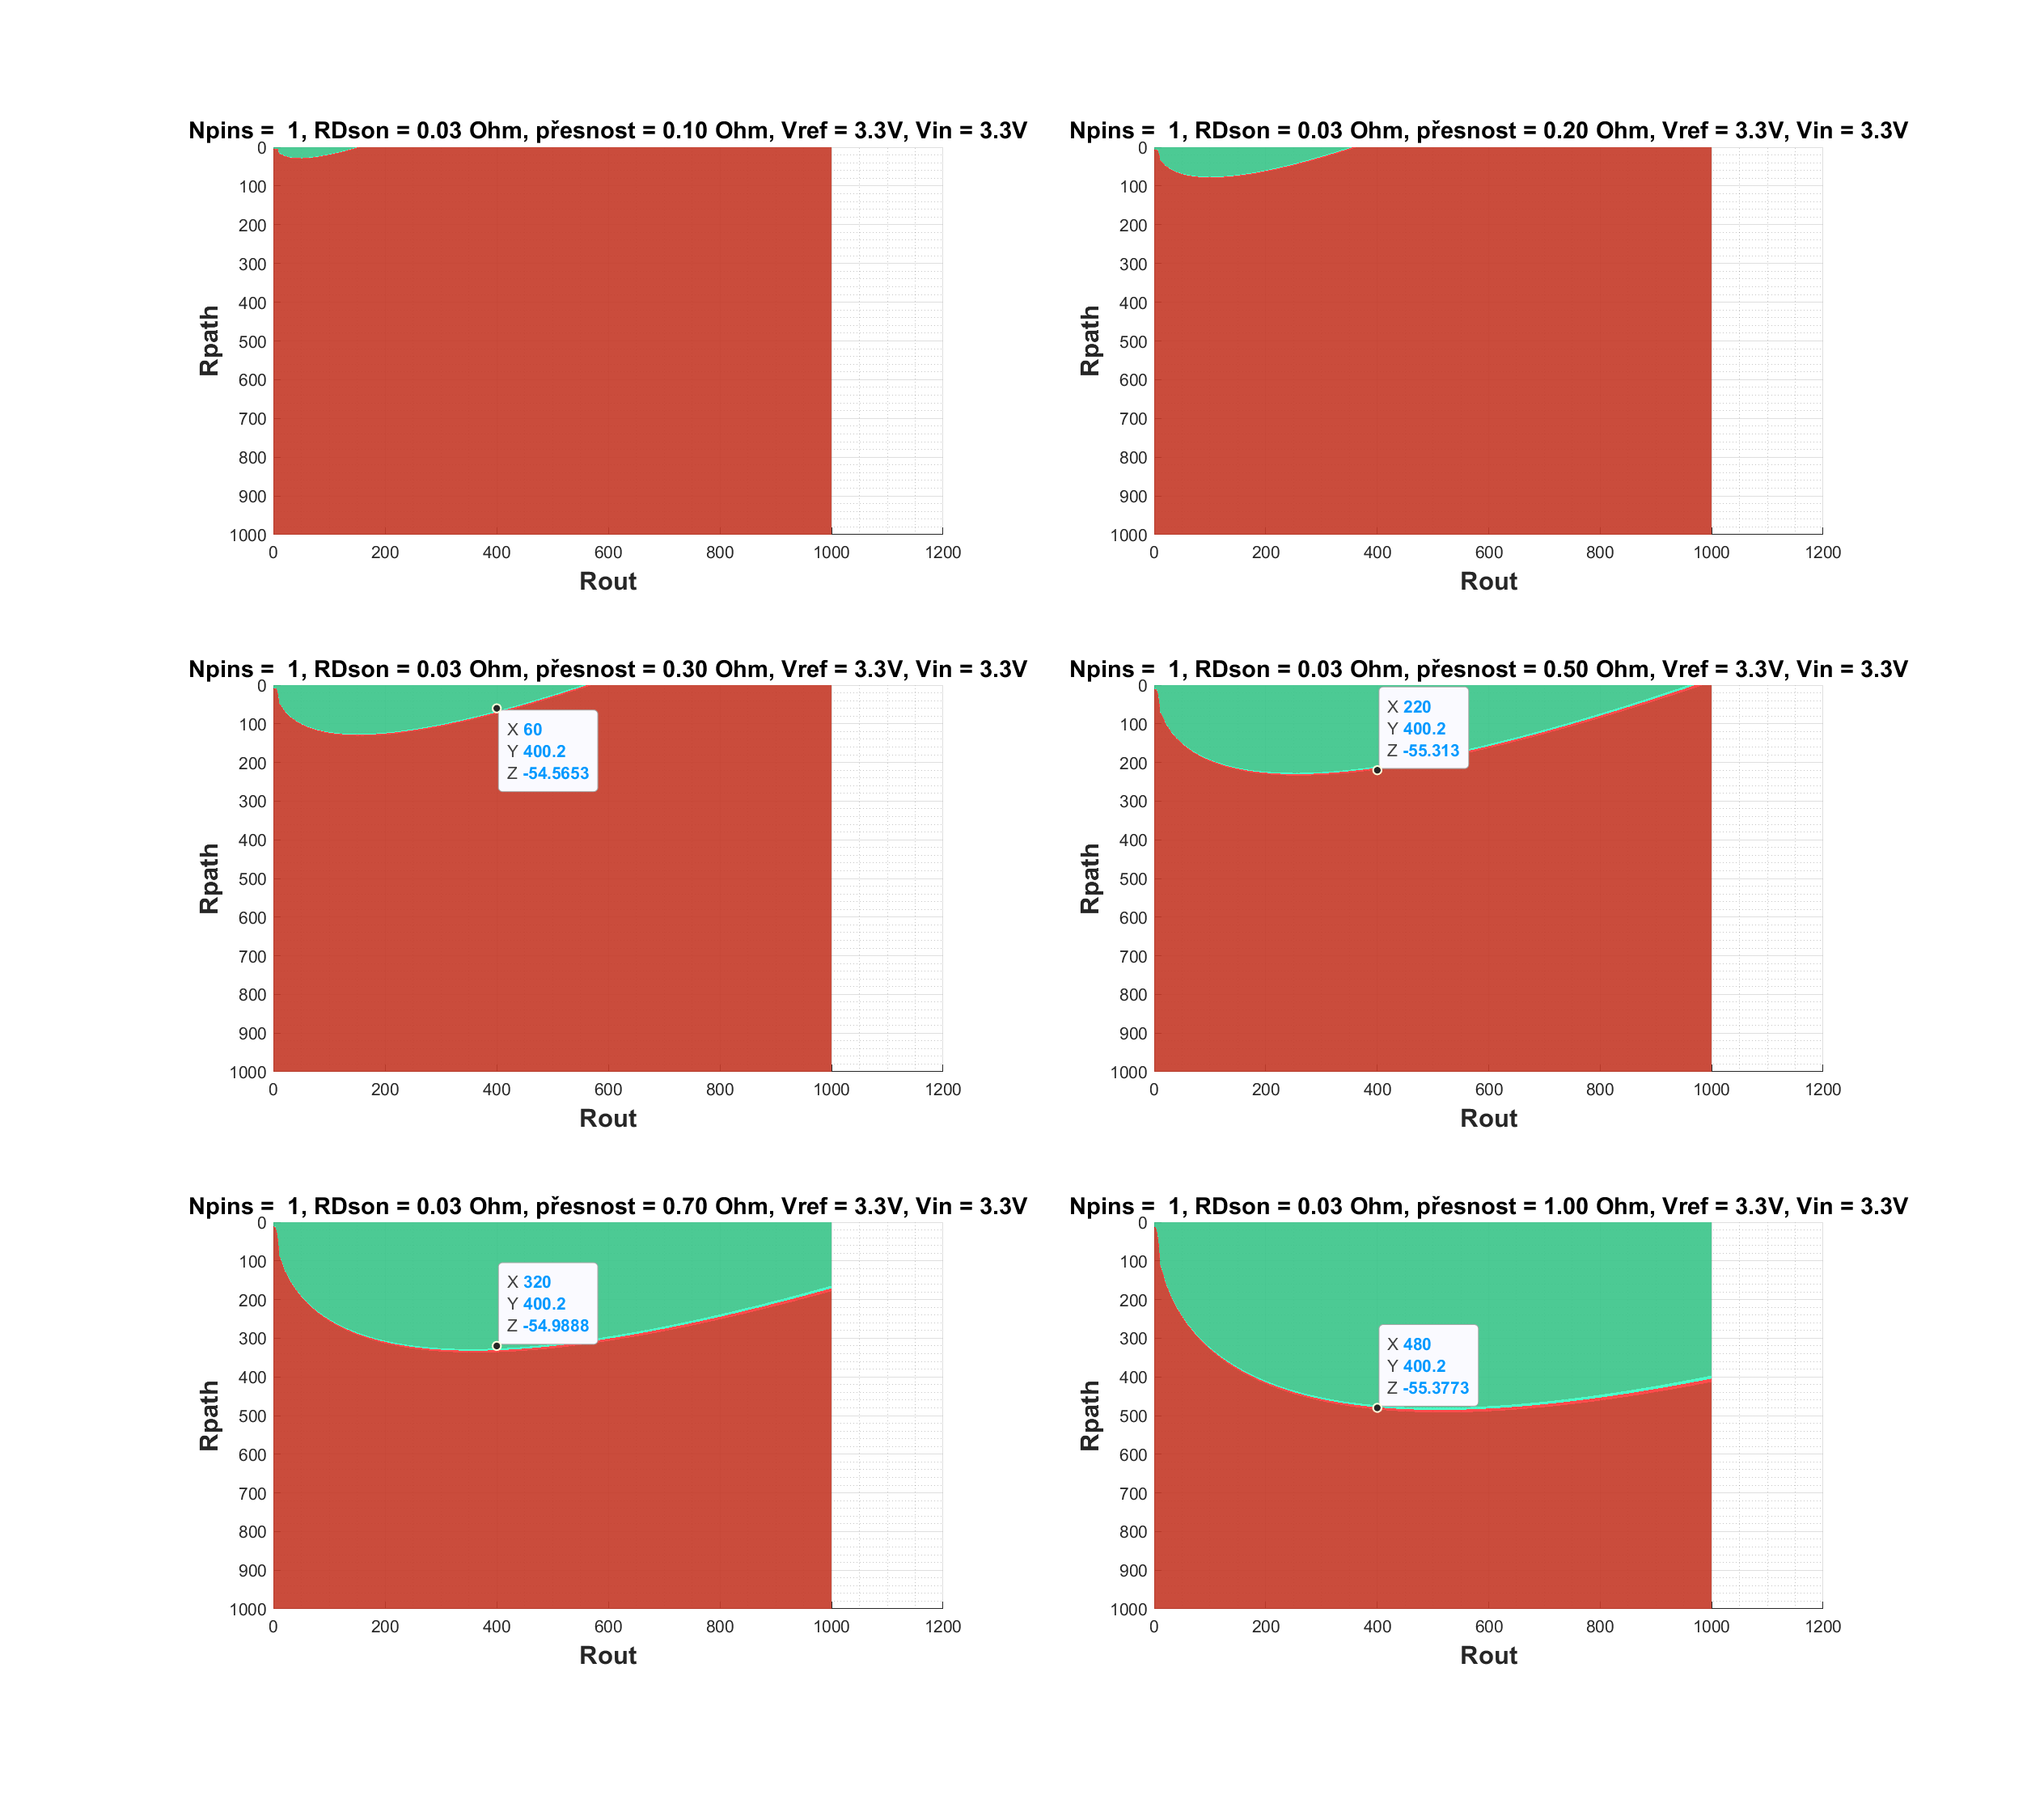
\includegraphics[height = 0.8\textheight]{obrazky/MERENI_JEDNOHO_PINU.eps}
		\end{minipage}
	\end{figure}
\end{frame}

\begin{frame} 
	% nadpis snímku
	\frametitle{Volba Rx: Vliv RDSON}
	\begin{figure}[ht!]
		\centering
		\begin{minipage}{0.3\textwidth}
			\begin{itemize}
				\item 40 pinů
				\item přesnost 2\,$\Omega$
				\item RDSON 15-35\,$m\Omega$
			\end{itemize}
		\end{minipage}
		\begin{minipage}{0.65\textwidth}
		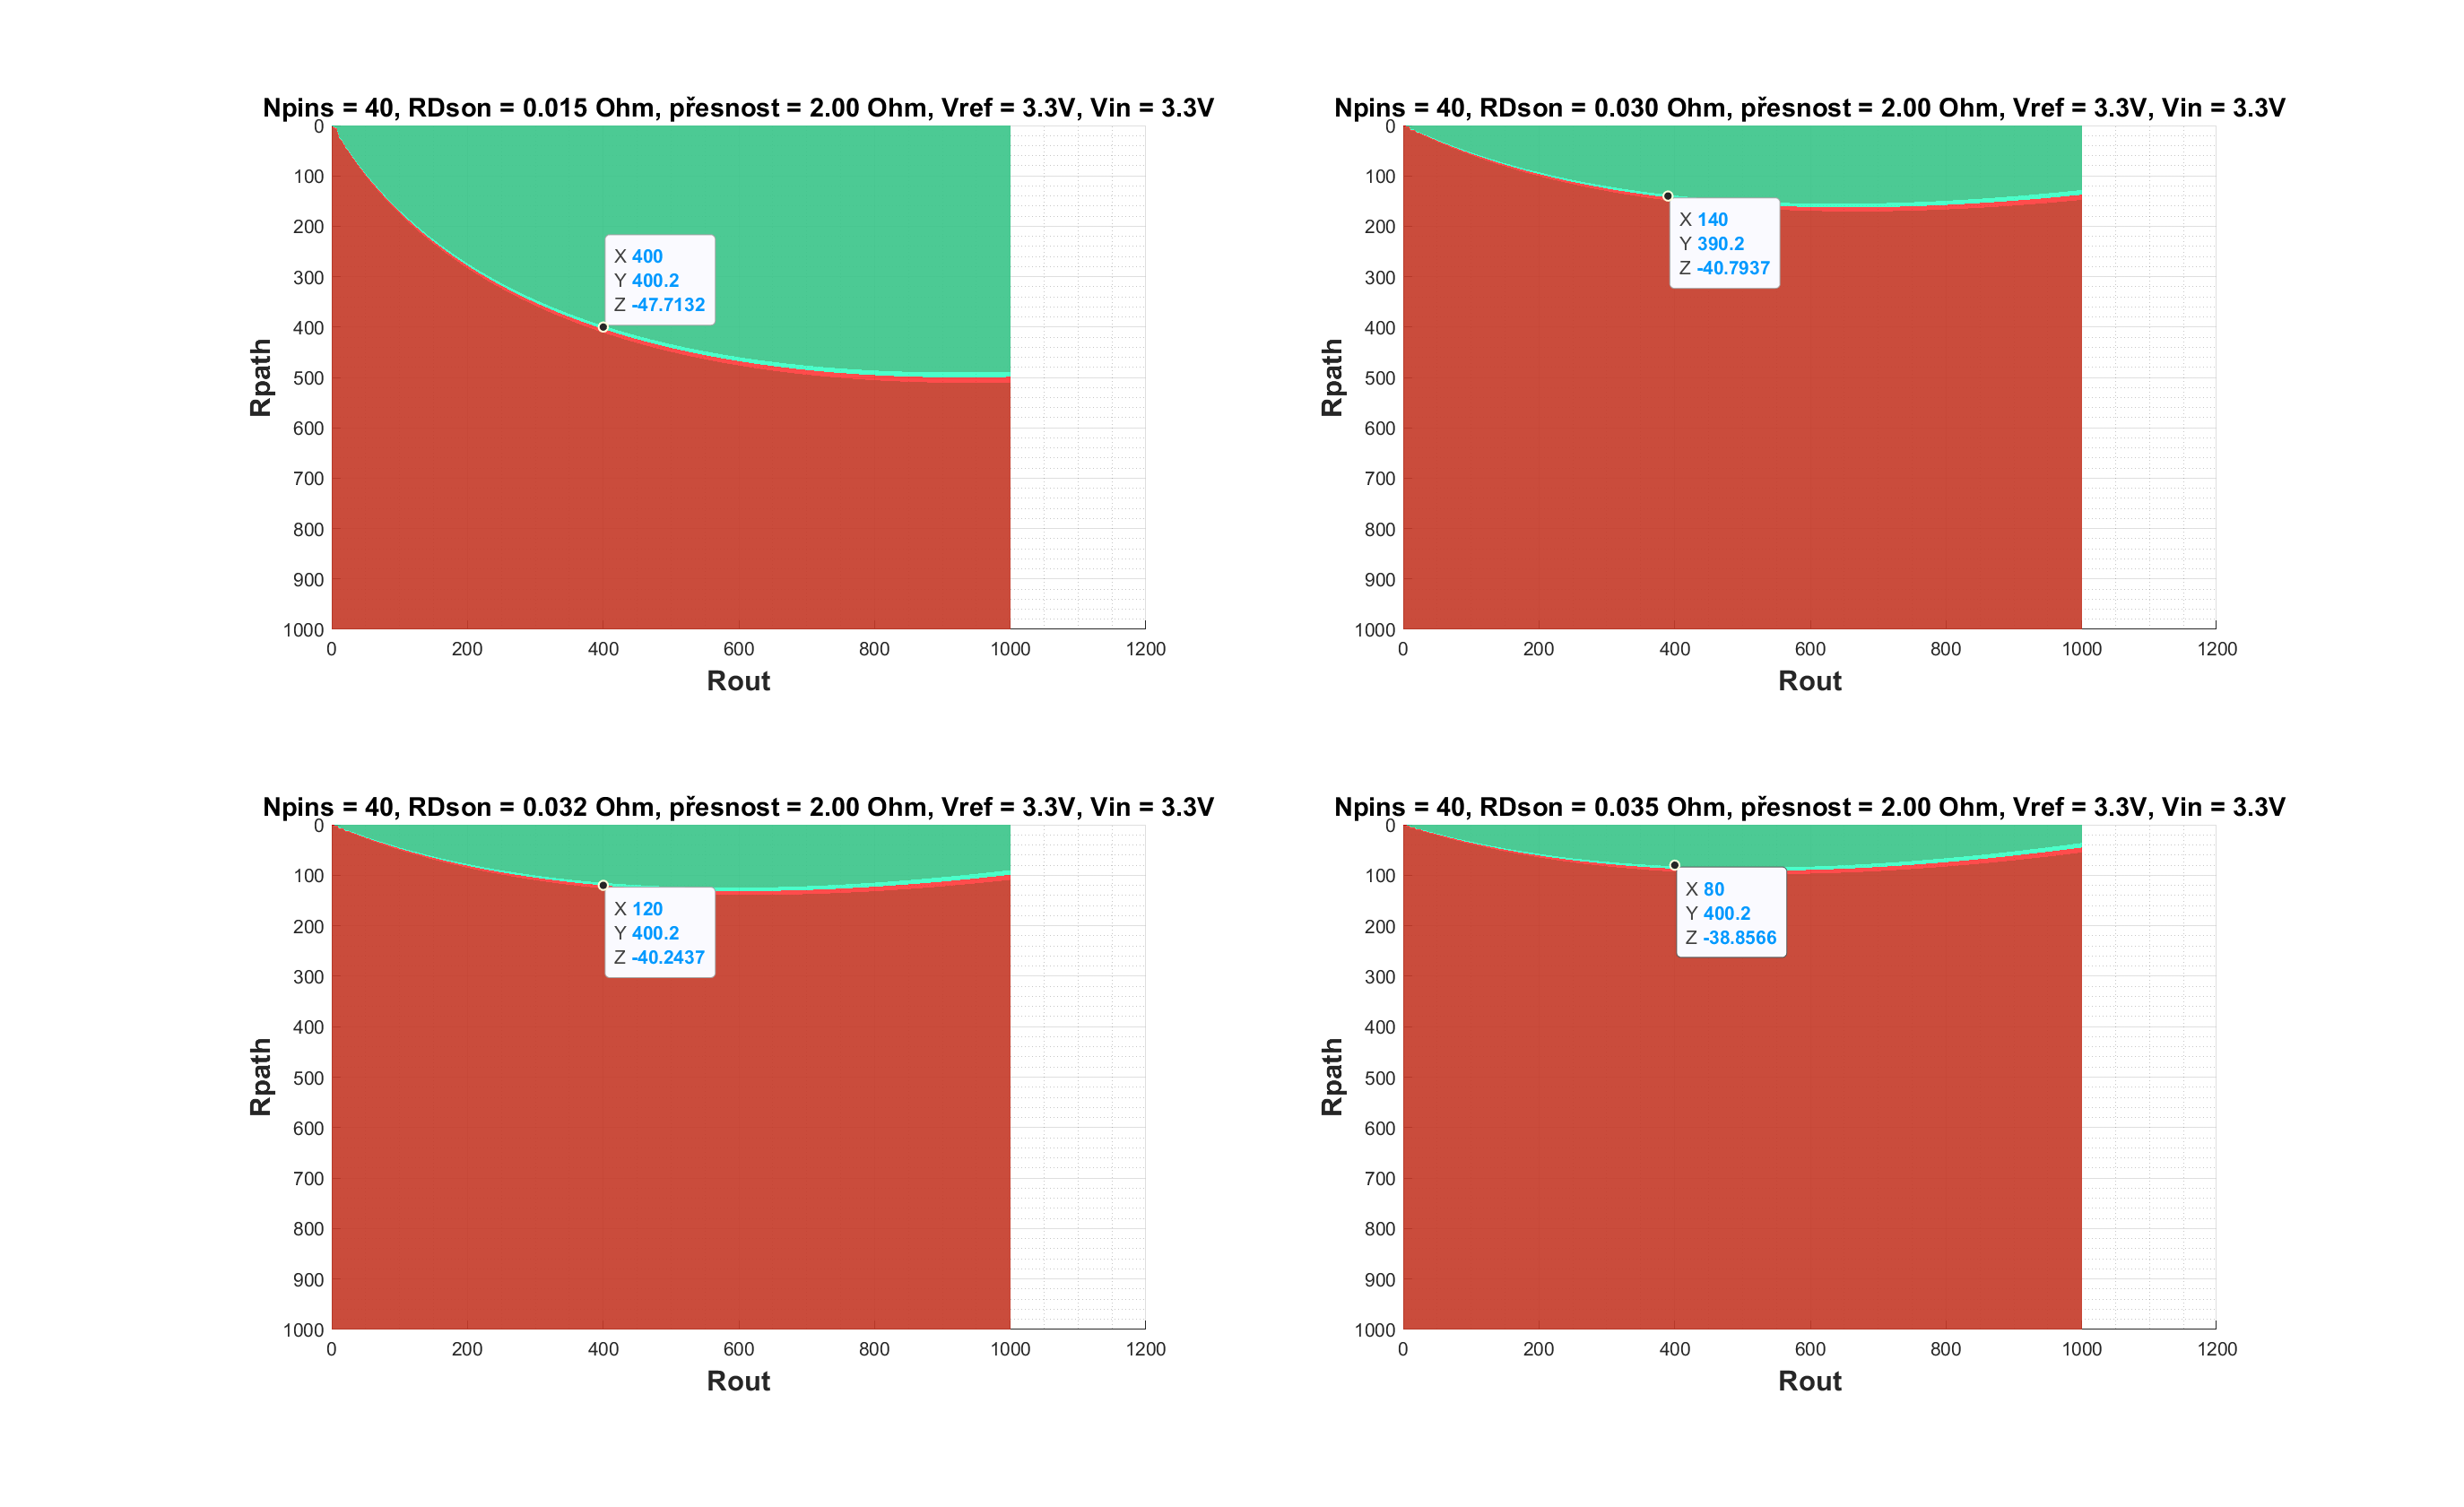
\includegraphics[width = 1.1\textwidth]{obrazky/vliv_RDSON.eps}
		\end{minipage}
	\end{figure}
\end{frame}


\begin{frame} 
	% nadpis snímku
	\frametitle{Ovládací karta}

	\begin{figure}[ht!]
		\centering
		%\includegraphics[width = \textwidth]{obrazky/system_connection.png}
		\includegraphics[height = 0.8\textheight]{obrazky/ovladaci_karta_diag.png}
	\end{figure}
\end{frame}


\begin{frame} 
	% nadpis snímku
	\frametitle{PC aplikace 1/2}

	\begin{figure}[ht!]
		\centering
		%\includegraphics[width = \textwidth]{obrazky/system_connection.png}
		\includegraphics[width = 0.85\textwidth]{obrazky/PC_AP_top_view.png}
	\end{figure}
\end{frame}

\begin{frame} 
	% nadpis snímku
	\frametitle{PC aplikace 2/2}

	\begin{figure}[ht!]
		\centering
		%\includegraphics[width = \textwidth]{obrazky/system_connection.png}
		\includegraphics[width = 0.85\textwidth]{obrazky/PC_AP_top_only1.png}
	\end{figure}
\end{frame}

%%%%%%%%%%%%%
\begin{frame} 
	\frametitle{Pokračování do DP}
	\vspace*{0.5cm}
	\begin{itemize}
		\item Osazení měřící karty a odladění firmwaru
		\item Dokončení návrhu a výroba ovládací karty
		\item Bezpečnostní prvky (RACK)
		\item Rozšíření PC aplikace
		\item Mechanická konstrukce testeru
		\item Ověření funkčnosti a parametrů
	\end{itemize}
\end{frame}


% podekovani
\begin{frame}[c] 
% bez nadpisu snímku
	\frametitle{\mbox{ }}
	\begin{center}
		{\Huge Děkuji za pozornost!}
	\end{center}
\end{frame}

% otázky oponenta
%frame{
%frametitle{Otázky oponenta}
%\begin{itemize}
%	\item \textbf{Otázka 1:}\\
%	Odpověď 1
%	\item \textbf{Otázka 2:}\\
%	Odpověď 2
%\end{itemize}
%

\end{document}
